\chapter{Semana 01 (02/02--04/02) --- Do Caos à Clareza}

\section{Intenção da aula (em 1 frase)}
Hoje eu vou mostrar, na prática, que \textbf{dados brutos são ruído} e que o valor profissional do aluno aparece quando ele consegue \textbf{limpar, entender e comunicar} os dados como uma história que leva a uma decisão.

\section{O que eu preciso ter pronto antes de entrar em sala}
\begin{itemize}[leftmargin=*]
  \item Um dataset exemplo (eu uso um CSV estilo \textit{Netflix Titles} para simular o fluxo). 
  \item Um notebook base com o esqueleto do ETL (leitura, inspeção, tipos, ausências, conversão de data, exportação).
  \item Tableau aberto (ou instalador) e o CSV \textit{limpo} para conectar ao vivo.
  \item O infográfico de fechamento: \texttt{info\_semana1.png} (quando existir) e o PDF da apresentação (você vai atualizar depois).
\end{itemize}

\section{Roteiro de 3 horas (19h--22h) \textemdash{} texto em 1\textsuperscript{a} pessoa}

\subsection*{19:00--19:20 \textemdash{} Abertura, Gancho e a Big Idea}
Eu começo reconhecendo o contexto real da turma:

\begin{BoardBox}
\textbf{Eu escrevo no quadro (bem grande):}

\vspace{4pt}
\textbf{Big Idea do semestre:}\\
\textit{``Dados brutos são apenas ruído; o seu valor no mercado será medido pela sua capacidade de extrair deles uma história que force uma decisão.''}
\end{BoardBox}

Eu digo que a disciplina não é sobre ``aprender ferramenta''. É sobre \textbf{mudar de postura}: sair do ``eu fiz um gráfico'' para ``eu provo uma conclusão''.

Eu lanço uma pergunta provocativa (para tirar a sala do modo passivo):

\begin{BoardBox}
\textbf{Pergunta para a turma:} 
\textit{``Por que algumas empresas sobrevivem a crises e outras não?''}

\textbf{Eu puxo para o próximo passo:}
\textit{``Não é falta de dados. É falta de perguntas certas e de leitura certa.''}
\end{BoardBox}

\subsection*{19:20--19:45 \textemdash{} AED vs Explanativa (cozinha vs jantar)}
Eu explico a diferença de intenção. Na AED eu quero \textbf{descobrir} (testar hipóteses, checar dados, procurar outliers). Na explanativa eu quero \textbf{convencer} (uma mensagem clara, com evidência).

Eu uso uma tabela, porque ela fica muito didática (e eu reaproveito no PDF depois):

\begin{center}
\renewcommand{\arraystretch}{1.2}
\begin{tabular}{@{}p{3.2cm} p{5.2cm} p{5.2cm}@{}}
\toprule
\textbf{Item} & \textbf{Análise Exploratória (A Cozinha)} & \textbf{Análise Explanativa (O Jantar)} \\
\midrule
Objetivo & Entender dados, encontrar padrões e anomalias & Comunicar insights e forçar uma decisão \\
Público & Eu (analista) & Gestão / cliente / time \\
Produto & Hipóteses, checagens, rascunhos & 1 mensagem central (Big Idea) + evidência \\
Ferramenta & Python / Pandas / Jupyter & Tableau / dashboard / apresentação \\
\bottomrule
\end{tabular}
\end{center}

Eu fecho esse bloco com uma regra prática:

\begin{BoardBox}
\textbf{Regra:} \textit{AED \=\= ``explorar sem medo''. Explanativa \=\= ``editar sem piedade''.}
\end{BoardBox}

\subsection*{19:45--20:45 \textemdash{} Mão na massa: ETL com Python (o caos controlado)}
Eu digo explicitamente o que vou fazer, para a turma enxergar o fluxo:

\begin{BoardBox}
\textbf{Fluxo de hoje (ETL):}\\
\textit{CSV bruto} $\rightarrow$ \textit{Pandas (ler/inspecionar)} $\rightarrow$ \textit{limpar/transformar} $\rightarrow$ \textit{exportar CSV limpo} $\rightarrow$ \textit{Tableau}
\end{BoardBox}

\subsubsection*{Passo 1 --- Extrair (ler e interrogar)}
Eu abro o notebook e não deixo a turma digitar tudo do zero ainda: primeiro eu mostro o raciocínio.

\begin{lstlisting}[language=Python,caption={Leitura inicial e inspeção (Extract)}]
import pandas as pd

df = pd.read_csv("netflix_titles.csv")

df.head()
df.shape

df.info()

df.isna().sum().sort_values(ascending=False).head(10)
\end{lstlisting}

Eu paro aqui e pergunto:
\begin{itemize}[leftmargin=*]
  \item \textbf{Quais colunas parecem promissoras para uma história?}
  \item \textbf{Quais colunas parecem "sujeira" para o nosso objetivo?}
  \item \textbf{Onde o dado pode nos enganar?} (missing, tipos errados, categorias sujas)
\end{itemize}

\subsubsection*{Passo 2 --- Transformar (limpar para não engasgar no Tableau)}
Eu foco em duas limpezas essenciais na primeira aula: \textbf{datas} e \textbf{colunas desnecessárias}.

\paragraph{2.1 Converter data (texto \textrightarrow{} datetime)}
Eu explico rapidamente por que isso importa:
\begin{itemize}[leftmargin=*]
  \item texto não ordena bem por tempo;
  \item não gera eixo temporal correto;
  \item vira dor de cabeça no Tableau.
\end{itemize}

\begin{lstlisting}[language=Python,caption={Converter datas e padronizar campos}]
# Exemplo: se existir coluna 'date_added'
df['date_added'] = pd.to_datetime(df['date_added'], errors='coerce')

# Exemplo: se existir coluna 'release_year' como numero OK; se vier como texto:
df['release_year'] = pd.to_numeric(df['release_year'], errors='coerce')
\end{lstlisting}

\paragraph{2.2 Missing: medir antes de agir}
Eu ensino a turma a não sair removendo tudo.

\begin{FormulaBox}
\textbf{Taxa de ausência (por coluna):}\quad
$\displaystyle \text{missing\_rate} = \frac{\#\text{nulos}}{n}$
\end{FormulaBox}

\begin{lstlisting}[language=Python,caption={Taxa de ausência e decisões iniciais}]
missing_rate = df.isna().mean().sort_values(ascending=False)
missing_rate.head(10)

# Exemplo de regra pragmatica (ajustar em aula):
# - se uma coluna tem > 80% missing e nao eh essencial, eu removo.
\end{lstlisting}

\paragraph{2.3 Remover colunas que não ajudam o objetivo (primeiro corte)}
Eu explico que colunas não são "boas" ou "ruins" sozinhas: elas são \textbf{boas para um objetivo}. Como hoje o objetivo é um primeiro dashboard, eu simplifico.

\begin{lstlisting}[language=Python,caption={Selecionar colunas essenciais para a primeira história}]
cols_keep = [
    'type', 'title', 'country', 'date_added',
    'release_year', 'rating', 'listed_in'
]

cols_keep = [c for c in cols_keep if c in df.columns]

df_clean = df[cols_keep].copy()
\end{lstlisting}

\paragraph{2.4 Normalização rápida de texto (categorias "sujas")}
Eu mostro um exemplo curto porque no mundo real isso sempre aparece:

\begin{lstlisting}[language=Python,caption={Limpeza simples de strings}]
for col in ['country', 'listed_in', 'rating', 'type']:
    if col in df_clean.columns:
        df_clean[col] = df_clean[col].astype(str).str.strip()
\end{lstlisting}

\subsubsection*{Passo 3 --- Load (exportar CSV limpo)}
Eu reforço que esse CSV limpo é o ``ingrediente'' que faz o Tableau voar.

\begin{lstlisting}[language=Python,caption={Exportar dataset pronto para Tableau}]
output_path = "netflix_limpo.csv"
df_clean.to_csv(output_path, index=False)
\end{lstlisting}

Eu fecho essa parte com um checklist, para eles internalizarem:

\begin{SolvedBox}
\textbf{Checklist de ETL (Semana 01):}
\begin{itemize}[leftmargin=*]
  \item Eu consigo explicar o que cada coluna significa?
  \item Eu sei quantos registros e quantas colunas tenho?
  \item Eu medi missing (antes de imputar/remover)?
  \item Eu converti datas para datetime quando existir data?
  \item Eu exportei um CSV limpo com colunas que suportam minha pergunta?
\end{itemize}
\end{SolvedBox}

\subsection*{20:45--21:00 \textemdash{} Intervalo}
Eu aproveito para circular e ver quem está travado em instalação/arquivo.

\subsection*{21:00--21:45 \textemdash{} Tableau: do dado limpo ao primeiro insight visual}
Aqui eu \textbf{simulo} a execução como eu faria em sala.

\subsubsection*{Passo a passo de conexão}
\begin{itemize}[leftmargin=*]
  \item Eu abro o Tableau e clico em \textbf{Text File} (Arquivo de Texto).
  \item Eu seleciono \texttt{netflix\_limpo.csv}.
  \item Eu confiro tipos: datas como data, anos como número, texto como dimensão.
\end{itemize}

\subsubsection*{Visual 1: mapa por país (quando existir country)}
Eu digo: "Eu quero sentir a distribuição".
\begin{itemize}[leftmargin=*]
  \item Eu arrasto \textbf{country} para a \textbf{view}.
  \item Se o Tableau reconhecer geografia, eu deixo como mapa.
  \item Se não reconhecer (por causa de países múltiplos em uma célula), eu explico o problema e prometo resolver em outra aula com split/normalização.
\end{itemize}

\subsubsection*{Visual 2: contagem por tipo (Movie vs TV Show)}
\begin{itemize}[leftmargin=*]
  \item Eu arrasto \textbf{type} para Rows.
  \item Eu arrasto \textbf{Number of Records} para Columns.
  \item Eu ordeno e adiciono rótulos.
\end{itemize}

\subsubsection*{Visual 3: linha no tempo (adições por mês/ano)}
\begin{itemize}[leftmargin=*]
  \item Eu arrasto \textbf{date\_added} para Columns.
  \item Eu arrasto \textbf{Number of Records} para Rows.
  \item Eu ajusto o nível da data (mês/ano) e mostro como isso muda a história.
\end{itemize}

\subsubsection*{Teste do Relance (3 segundos) \textemdash{} regra de design}
Eu explico que um visual pode estar certo e ainda assim ser ruim (porque não comunica). Então eu aplico o Teste do Relance.

\begin{BoardBox}
\textbf{Teste do Relance (3s):}
\begin{itemize}[leftmargin=*]
  \item O título diz a \textbf{mensagem} (não o tipo de gráfico)?
  \item Eu sei o que comparar sem ler uma legenda complexa?
  \item O gráfico tem ruído visual (grades, cores desnecessárias)?
\end{itemize}
\end{BoardBox}

Eu faço 2 ajustes em tempo real (para mostrar impacto): remover grades, deixar 1 cor principal + 1 cor de destaque, e trocar título.

\subsection*{21:45--22:00 \textemdash{} Fechamento: o ``New Bliss'' + chamada para ação}
Eu fecho com uma cena futura (para engajar): o aluno abrindo um dashboard e calando a sala com evidência.

Eu finalizo com o que precisa ficar na cabeça deles:
\begin{BoardBox}
\textbf{Eu fecho assim:}
\textit{``Vocês não serão pagos por gráficos. Vocês serão pagos por decisões melhores.''}
\end{BoardBox}

\subsection*{O meu slide/infográfico de resumo (ao final)}
Eu mostro o infográfico final da aula (você vai colocar o arquivo depois).

\begin{NoteBox}
Se o arquivo \texttt{info\_semana1.png} existir em \texttt{aed/aula/semana01/}, ele aparece abaixo.
\end{NoteBox}

\begin{center}
\IfFileExists{semana01/info_semana1.png}{
  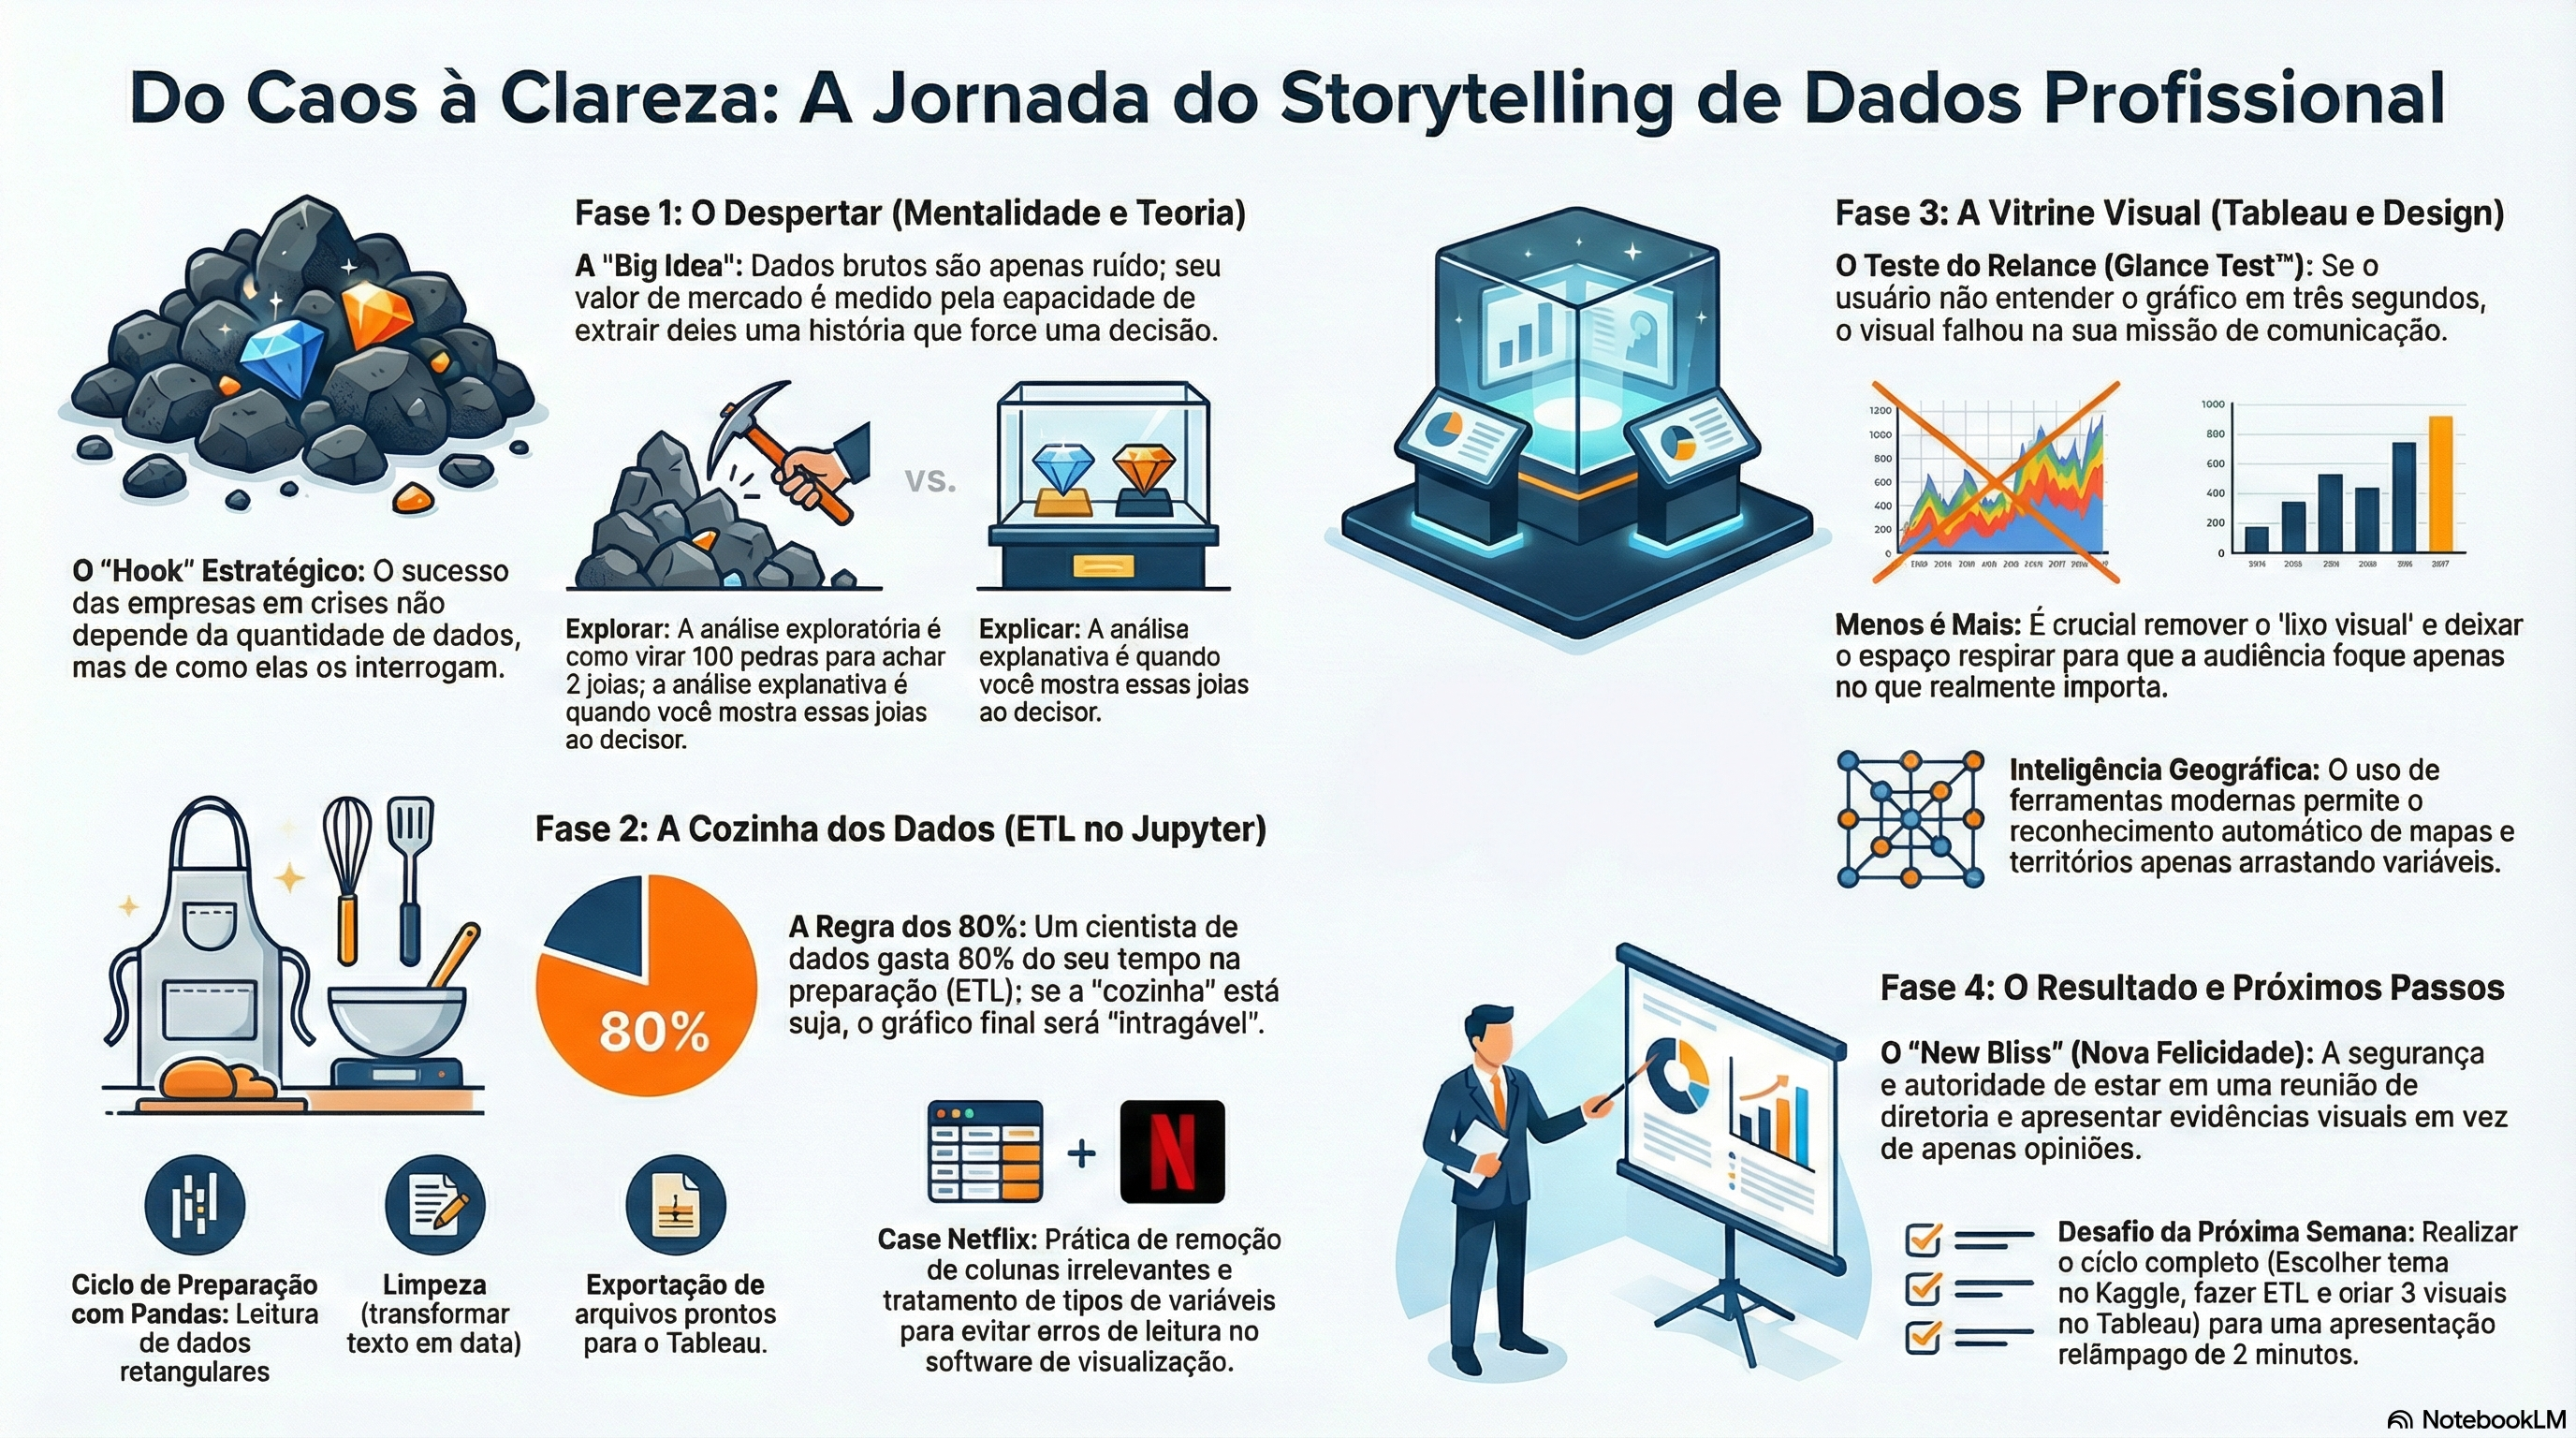
\includegraphics[width=0.92\textwidth]{semana01/info_semana1.png}
}{
  \fbox{\parbox{0.9\textwidth}{\centering \textit{(placeholder)}\quad Coloque aqui o arquivo \texttt{info\_semana1.png} em \texttt{aed/aula/semana01/}.}}
}
\end{center}

\section{Trabalho 1 (entrega na Semana 02) \textemdash{} 0,5 ponto na I unidade}
\subsection*{Objetivo pedagógico}
Cada aluno escolhe um tema e, além de \textbf{construir um infográfico}, ele precisa \textbf{estudar um pouco o assunto} (livro, PDF, artigos) e ensinar a turma em 10 minutos. 

\begin{SolvedBox}
\textbf{Formato (Semana 02):} cada aluno tem \textbf{10 minutos}.
\begin{itemize}[leftmargin=*]
  \item 7 min: construir/mostrar o infográfico (Tableau) e explicar a Big Idea.
  \item 3 min: explicar o que estudou (conceito) e responder 1 pergunta.
\end{itemize}

\textbf{Entregáveis:}
\begin{itemize}[leftmargin=*]
  \item 1 CSV (dataset escolhido) e 1 CSV limpo (separado);
  \item 1 notebook (ETL básico com evidência de limpeza real);
  \item 1 visual/infográfico no Tableau;
  \item 1 slide (ou texto curto) com \textbf{Big Idea} + 3 bullets de evidência.
\end{itemize}
\end{SolvedBox}

\subsection*{Os 20 temas (para eu mostrar no final da Semana 01)}
Eu apresento a lista e deixo claro: tema não é ``qualquer dataset''; tema é \textbf{uma pergunta + um recorte + um conceito para estudar}.

\begin{center}
\renewcommand{\arraystretch}{1.2}
\begin{tabular}{@{}c p{4.3cm} p{5.0cm} p{4.0cm}@{}}
\toprule
\textbf{\#} & \textbf{Tema (assunto)} & \textbf{Pergunta/recorte (para o infográfico)} & \textbf{Conceito para estudar} \\
\midrule
01 & Netflix: produções por ano & Houve crescimento? quais anos mudam o ritmo? & Eixo temporal e granularidade \\
02 & Netflix: filme vs série & Qual tipo domina? muda por ano? & Proporções e comparação \\
03 & Netflix: países mais presentes & Quais países lideram? e por quê? & Categóricas + limpeza de texto \\
04 & Netflix: classificação indicativa & Quais ratings mais comuns? & Distribuição categórica \\
05 & Netflix: gêneros (listed\_in) & Top gêneros e combinações & Categorias ``multivalor'' \\
06 & Vendas de videogames & Quais plataformas/regiões lideram? & Grupos e comparação \\
07 & Filmes (IMDb/TMDB) & Orçamento vs receita: existe relação? & Scatter e correlação (noção) \\
08 & Airbnb (NY) & Bairro vs preço: onde é mais caro? & Boxplot e dispersão \\
09 & Preços de abacate & Sazonalidade: meses mais caros? & Séries temporais \\
10 & Felicidade mundial & PIB vs felicidade: padrão global? & Correlação \neq causalidade \\
11 & Salários em Data Science & Senioridade vs salário: qual salto? & Segmentação por categoria \\
12 & Reviews e-commerce & Nota vs recomendação: o que pesa? & Viés de seleção \\
13 & Starbucks nutrição & Calorias vs tamanho: onde está o pico? & Outliers e interpretação \\
14 & Qualidade do vinho & \% álcool vs qualidade: há tendência? & Relação bivariada \\
15 & Diabetes (Pima) & Glicose vs diagnóstico: separa grupos? & Comparar distribuições \\
16 & Crimes (cidade) & Horário/dia: onde estão os picos? & Heatmap simples \\
17 & Apps (Google Play) & Avaliação vs installs: existe padrão? & Escalas e log (noção) \\
18 & Temperatura global & Tendência: aquecimento aparece? & Linha do tempo e smoothing \\
19 & Spotify top hits & BPM vs popularidade: existe relação? & Dispersão e clusters \\
20 & Titanic & Sobrevivência por classe/sexo: qual diferença? & Proporções e narrativa \\
\bottomrule
\end{tabular}
\end{center}

\begin{NoteBox}
Eu deixo o aluno escolher um tema, mas eu cobro que ele traga \textbf{uma Big Idea} e \textbf{uma evidência} (não apenas um gráfico bonito). Eu reforço que o objetivo é ensinar a turma.
\end{NoteBox}

\section{Referências (para eu citar e orientar leitura)}
Eu menciono explicitamente os materiais e deixo a turma saber que eles vão reaparecer na unidade:
\begin{itemize}[leftmargin=*]
  \item Estatística prática e AED (base): \cite{bruce_estatistica_pratica}.
  \item Storytelling (clareza, Big Idea, persuasão): \cite{duarte_datastory}.
  \item Apostila/guia LaTeX (conteúdos e exercícios): \cite{unifacol_apostila_aed}.
\end{itemize}
